% \chapter{Long Title}{Short Title}
% The Long Title will appear on the first page of the chapter.
% The Short Title will appear in the table of contents.
% If the Long Title isn't all that long, you can just call
% \chapter{Long Title}{} and the same title will appear in
% both places.


\chapter{Multivariate moment problems and the Radon transform}{}

\section{Classical and multivariate moment mroblems}
Let $f(x)$ be a measurable function on $\RR$. For $k \in \NN_0$, define the $k$th moment of $f$ as
\[
  c_k = \int_{-\infty}^\infty f(x)x^k ~dx.
\]
The sequence ${(c_k)}_{k \in \NN_0}$ is called a moment sequence or a moment problem, and the function $f$ is called a solution to the moment problem. Loosly speaking a moment problem poses the question: Under given constraints (e.g.\ domain, continuity, etc\ldots), to what extent can one determine the solution $f$ from its moments?

The classical study of moment problems is divided into three cases depending on the domain: 
\begin{enumerate}
  \item Markov (or Haussdorf) moment problems for bounded domains (i.e.\ the unit interval), 
  \item Stieltjes moment problems for one-sided unbounded domains (i.e.\ the positive real line), and 
  \item Hamburger moment problems for bi-infinite domains (i.e.\ the real line).
\end{enumerate}

There are two natural questions one can ask about a moment problem:
\begin{enumerate}
  \item Solvability: Does a solution $f$ exist possessing the given moments?
  \item Determinacy: Is a solution unique? If not, what can be said about the set of solutions?
\end{enumerate}
In the classical cases (Markov, Stieltjes, Hamburger) these questions have been resolved. Precise conditions for solvable and determinate moment problems exist, and the nature of solution sets to indeterminate moment problems are well understood. For instance, in the class of continuous functions on the unit interval, all solvable moments problems are determinate. However many classes of generalized moment problems remain in active study.

In particular let us discuss multivariate moment problems. Let $f(x)$ be a measureable function now on $\RR^n$. For $\alpha \in \NN_0^n$, define the $\alpha$th multivariate moment of $f$ as 
\[
  c_\alpha = \int_{\RR^n} f(x)x^\alpha ~ dx.
\]
The moment sequence ${(c_\alpha)}_{\alpha \in \NN_0^n}$ is now multiindexed. No precise general conditions are known for the solvability or determinacy of multivariate moment problems. However some sufficient conditions have been discovered by leveraging classical moment problem theory~\cite{Pete82}.

\begin{myexample}
  Let $A = {[0,1]}^n \subseteq \RR^n$ be the unit cube and $f$ its characteristic function. Then $f$ has multivariable moments
  \begin{align*}
    \int_{\RR^n} f(x) x^\alpha ~dx 
    % &= \int_A x_1^{\alpha_1}x_2^{\alpha_2} \cdots x_n^{\alpha_n} dx \\
    % &= \int_0^1 \int_0^1 \cdots \int_0^1 x_1^{\alpha_1}x_2^{\alpha_2} \cdots x_n^{\alpha_n} ~dx_1~dx_2\cdots~dx_n \\
    &= \int_0^1 x_1^{\alpha_1} ~dx_1 \int_0^1 x_2^{\alpha_2} ~dx_2 \cdots \int_0^1 x_n^{\alpha_n} ~dx_n \\
    &= \frac{1}{(\alpha_1+1) (\alpha_2+1) \cdots (\alpha_n+1)}
  \end{align*}
  Similarly for any rectanglular region $A = \prod_{i = 1}^n [a_i, b_i]$
  \[
    \int_A x^\alpha ~dx 
    = \prod_{i=1}^n \int_{a_i}^{b_i} x_i^{\alpha_i}
    = \prod_{i = 1}^n \frac{b_i^{\alpha_i + 1} - a_i^{\alpha_i + 1}}{\alpha_i + 1}
  \]
\end{myexample}


\section{Gaussian functions and measures}
\begin{definition}
  Let $w(p) : \RR \rightarrow \RR$  be the standard Gaussian density on $\RR$,
  \[
    w(p) = \frac1{\sqrt{2\pi}} e^{\frac{-p^2}2}
  \]
  and $w_n(x) : \RR^n \rightarrow \RR$ the standard Gaussian density on $\RR^n$,
  \[
    w_n(x) = {(2\pi)}^{-\frac n2} e^{\frac{-\|x\|^2}2}.
  \]
  Note that $w = w_1$.
\end{definition}

A couple of formula: First the Gaussian integral,
\[
  \int_{-\infty}^\infty w(p) ~dp = 1.
\]
This can be proven in a number of clever ways.

Second: The derivative
\[
  w'(p) = -pw(p).
\]

Third: The Gaussian function dominates polynomials in the sense that
\[
  \lim_{p \rightarrow -\infty} P(p)w(p) = 0 = \lim_{p \rightarrow \infty} P(p)w(p)
\]
for any polynomial $P$.

\begin{definition}
  The \textit{Gaussian moments} of a function $f: \RR^n \rightarrow \RR$ are
  \[
    c^G_\alpha = \int_{\RR^n} f(x)x^\alpha w(x) ~dx
  \]
  for $\alpha \in \NN_0^n$.
\end{definition}

\begin{myexample}
  Let $f: \RR \rightarrow \RR$ be the constant function $f(p)=1$. The Gaussian moments of $f$, i.e.\ the moments of $w(p)$, are
  \[
    c^G_k 
    = \begin{cases}
        (k-1)!!, & k~\text{even} \\
        0, & k~\text{odd}
    \end{cases}
  \]
  We have already seen $c_0 = 1$. Furthermore it is not hard to see that for odd $k$, 
  \[
    c^G_k = \int_{-\infty}^\infty p^k w(p) ~dp = 0
  \]
  since $p^k w(p)$ is an odd function.

  Now for $k \geq 2$ even, we derive a recurrence by integrating by parts
  \begin{align*}
    c^G_k
    &= \int_{-\infty}^\infty p^k w(p) ~dp \\
    &= -\int_{-\infty}^\infty p^{k-1} \left(-p w(p)\right) ~dp \\
    &= - \left[p^{k-1} w(p)\right]_{-\infty}^\infty + (k-1)\int_{-\infty}^\infty p^{k-2} w(p) ~dp \\
    &= (k-1)c^G_{k-2}.
  \end{align*}
  Thus by induction,
  \[
    c^G_k = (k - 1)(k - 3) \cdots c_0 = (k-1)!!.
  \]
\end{myexample}


A relationship between the univariate and multivariate Gaussian densities can be seen as follows: Let $x, y \in \RR^n$, $n \geq 2$. Suppose $y = p\omega$ where $\omega \in S^1$ and $p \in \RR$, so that $p\omega$ is the orthogonal projection of $x$ onto the span of $y$. Then the Pythagorean relation,
\[
  \|x\|^2 = \|x - p\omega\|^2 + \|p\omega\|^2 = \|x - p\omega\|^2 + p^2
\]
implies that
\begin{align*}
  w_n(x) 
  &= {(2\pi)}^{-\frac n2} e^{\frac{-\|x\|^2}2} \\
  &= {(2\pi)}^{-\frac{n-1}2} e^{\frac{-\|x - p\omega\|^2}2} {(2\pi)}^{-\frac12} e^{\frac{-p^2}2} \\
  &= w_{n-1}(x - p\omega)w(p)
\end{align*}
The equation
\begin{equation}\label{eq:gaussPythag}
  w_n(x) = w_{n-1}(x - p\omega)w(p)
\end{equation}
is in some respect the defining property of the Gaussian measure described below. Indeed if $x = (x_1, x_2, \ldots, x_n)$, by repeated application of (\ref{eq:gaussPythag}) one can write the decomposition
\[
  w_n(x) = \prod_{k = 1}^n w(x_k).
\]
Thus the $w_n(x)$ is the product of $n$ copies of $w$. The standard Gaussian measure $\gamma^n$ is thus a measure whose cardinal projections are standard Gaussian measures.

\begin{definition}
Let $\gamma^n$ be a the Borel measure on $\RR^n$ with density $w_n$,
\[
  \int_{\RR^n} f(x) d\gamma^n = \int_{\RR^n} f(x) w_n(x) ~dx.
\]
We call $\gamma^n$ the \textit{standard Gaussian measure}. 
More generally, for mean $a \in \RR^n$, and variance $\sigma > 0$, the following $\gamma^{n}_{a, \sigma^2}$ are \textit{Gaussian measures},
\begin{align*}
  \int_{\RR^n} f(x) d\gamma^n_{a,\sigma^2}
  &= \frac{{(2\pi)}^{-\frac n2}}{\sigma}  \int_{\RR^n} f(x) e^{-\frac{\|x - a\|^2}{2\sigma^2}} ~dx \\
  &= \int_{\RR^n} f(\sigma x + a) d\gamma^n
\end{align*}
% (Most general defn of Gaussian measures includes degenerate $\delta$ functions, and any product of Gaussian measures).
\end{definition}

\begin{myexample}
  Let $f:\RR^n \rightarrow \RR$ be the constant function $f(x)=1$. The Gaussian moments of $f$ are the multivariate moments of $w_n(x)$, and can be written as
  \begin{align*}
    c^G_\alpha 
    &= \int_{\RR^n} x^\alpha w_n(x) ~dx \\
    &= \prod_{\ell = 1}^n \int_{-\infty}^\infty x_\ell^{\alpha_\ell} w(x_\ell) ~dx \\
    &= \prod_{\ell = 1}^n c^G_{\alpha_\ell}
  \end{align*}
  where $\{c_k\}_{k \in \NN}$ are the univariate moments of $w(p)$.
  Thus $c^G_\alpha = 0$ if any $\alpha_i$ is odd. Otherwise, if every $\alpha_i$ is even then
  \[
    c^G_\alpha = \prod_{\ell = 1}^n (\alpha_\ell - 1)!!
  \]
\end{myexample}

\begin{definition}
  The \textit{Hermite polynomials} can be defined by the Rodriguez formula
  \[
      H_k(p) = {(-1)}^k \frac{w^{(k)}(p)}{w(p)}
  \]
  note that $H_k$ is a polynomial of degree $k$.
\end{definition}
The Hermite polynomials have the following properties:

\begin{align*}
  \int_{-\infty}^\infty H_k(p) H_\ell(p) w(p)~dp 
  = \begin{cases}
    \sqrt{2\pi} k!, & k = \ell \\
    0, & k \neq \ell
  \end{cases}
\end{align*}


\section{The Radon and Gaussian Radon transforms}

Let $f$ be a multivariable function on the $n$-dimensional Euclidean space $\RR^n$. We imagine taking ``slices'' of $f$ by restricting it to a $(n-1)$-dimensional hyperplane $\Lambda$. These hyperplanes form the domain of the Radon Transform. More precisely, the Radon Transform associates each slice with a corresponding integral
\[
  R_f(\Lambda) = \int_{\Lambda} f(x) ~dx,
\]
which can be thought of as a $(n-1)$-dimensional measurement of $f$. To be more precise we parametrize the collection of hyperplanes $\Lambda$ by normal vector, $\omega \in S^{n-1}$, and (signed) distance from the origin $-\infty < p < \infty$. Indeed any hyperplane can be described in the form $\Lambda = \{x \in \RR^n: \langle x, \omega\rangle = p\}$. As mentioned, there is a slight inconsistency in these definitions where a hyperplane $\Lambda$ can be indexed by both $\langle \omega, x \rangle = p$ and $\langle -\omega, x \rangle = -p$. This difference is inconsequential for our purposes so we choose the latter definition for clarity.

The Radon transform~\cite{Helg65} (RT) is a thing that I will discuss the history of, with references, in this paragraph. The transform gets its name from Johann Radon, whose first defined the tranform in the form below in 1917, although a similar transform was introduced by Paul Funk in 1911~\cite{????}. It is interesting to note that the primary application of the RT in medical imaging (CT scans) was not invented for another half century. I can only hope that in 2076 my dissertation will serve as an absorbant coffee coaster for a sleep deprived student.

\begin{definition}
  Let $f$ be a nonnegative measurable function on $\mathbb{R}^n$. The \textit{Radon transform} $R_f : S^{n-1} \times \RR \rightarrow \RR$ of $f$ is a function which, given a unit vector $\omega \in \RR^n$ and $-\infty < p < \infty$, is defined as
  \[
    R_f(\omega, p) = \int\mclimits_{\langle x, \omega \rangle = p} f(x) ~dx,
  \]
  provided the integral converges.
\end{definition}

\begin{myexample}
  For computation it is convenient to write the Radon Transform with an explicit isometric parameterization $x(t)$ of the hyperplane $\langle x, \omega\rangle = p$. In particular we note that there exists a map $x : \RR^{n-1} \rightarrow \RR^n$ such that $x(0) = p\omega$ and
  \[
    R_f(\omega, p) = \int_{\RR^{n-1}} f(x(t)) dt.
  \]

  For reference let's specify an hyperplane parameterization for the $n=2$ case. In $\RR^2$ often we identify $\omega$ with the angle $0 \leq \theta < 2\pi$ such that $\omega = (\cos \theta, \sin \theta)$. We define $x(t)$ by
  \begin{align*}
    x(t) = (t \sin \theta + p \cos \theta, -t \cos \theta + p \sin \theta), \qquad -\infty < t < \infty.
  \end{align*}
  It is not difficult to show that $x(0) = p\omega$, $\langle x(t), \omega \rangle = p$, and most importantly
  \[
    R_f(\omega, p) = \int_{-\infty}^\infty f(t \sin \theta + p \cos \theta, -t \cos \theta + p \sin \theta)~dt
  \]
\end{myexample}

\begin{myexample}
  Let $B(r) = \{x : |x| \leq r\} \subseteq \RR^n$ be the ball of radius $r$.
  \[
    R_{B(r)}(\omega, p) = 
    \begin{cases}
      V_{n-1}\left(\sqrt{r^2 - p^2}\right), & |p| \leq r \\
      0 & |p| > r
    \end{cases}    
  \]
  where $V_n(r)$ is the volume of a hypersphere of radius $r$,
  \[
    V_n(r) = \frac{\pi^{n/2}}{\Gamma(\frac n2+1)} r^n.
  \]
  Note that as a bounded domain, we can guarentee $B(r)$ is integrable on all hyperplanes. In fact the RT of any subset of $B(r)$ is sharply bounded by $R_{B(r)} \leq V_{n-1}(r)$. Also note that $B(r)$ is rotation invariant, hence $R_{B(r)}(\omega, p)$ is independent of $\omega$.
  
  \begin{figure}[h]
    \centering
    \includegraphics[width=0.7\textwidth]{Images/Ball RT.png}
    \caption{The RT of a ball}\label{fig:RTBall}
  \end{figure}

  We can use this formula to determine the RT of an anulus. Let $A(r_1, r_2) = \{x \in \RR^n: r_1 \leq \|x\| \leq r_2\}$. Then
  \begin{align*}
    R_{A(r_1, r_2)}(\omega, p) 
    &= R_{B(r_2)}(\omega, p) - R_{B(r_1)}(\omega, p) \\
    &= 
    \begin{cases}
      V_{n-1}(\sqrt{r_2^2 - p^2}) - V_{n-1}(\sqrt{r_1^2 - p^2}), & |p| < r_1 \\
      V_{n-1}(\sqrt{r_2^2 - p^2}), & r_1 \leq |p| \leq r_2 \\
      0, & |p| \geq r_2
    \end{cases}
  \end{align*}
\end{myexample}



Now consider an example of an unbounded region.

\begin{myexample}
Let $S = \{(x,y) : |y| \leq \frac12\} \subseteq \RR^2$ be a strip centered on the $x$-axis with width $1$. Clearly if $\theta = \pi/2$ or $3\pi/2$ then 
\[
  R_S(\theta, p) = 
  \begin{cases}
      \infty, & |p| \leq \frac12 \\
      0, & |p| > \frac12
  \end{cases}.
\]
Otherwise, 
\[
  R_S(\theta, p) = \sec \theta
\]
Note because $S$ is unbounded, that $R_S$ is not only unbounded, but even divergent in some cases.

\begin{figure}[h]
  \centering
  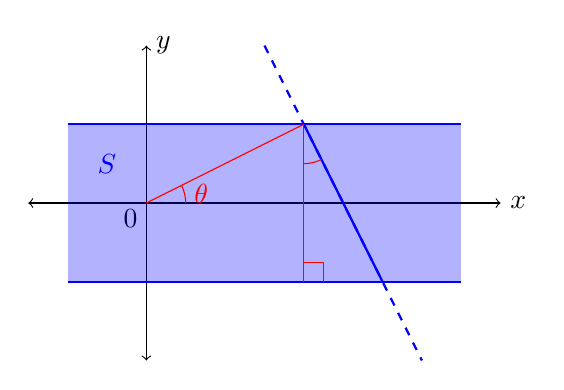
\begin{tikzpicture}[strip/.style={blue, fill=blue, fill opacity = 0.3},
      angle/.style={red},
      axis/.style={<->,black}]
  %draw axes
  \draw[axis] (-1.5,0) -- (4.5,0) node[anchor=west]{$x$};
  \node at (-.2,-.2) {$0$};
  \draw[axis] (0,-2) -- (0,2) node[anchor=west]{$y$};
  %draw wedge
  \fill[strip] (-1, 1) -- (4,1) -- (4, -1) -- (-1, -1) -- cycle;
  \draw[thick, blue] (-1,1) -- (4,1);
  \draw[thick, blue] (-1,-1) -- (4,-1);
  \node[blue] at (-0.5,0.5) {$S$};
  %draw hyperplane
  \draw[thick, blue, dashed] (1.5,2) -- (3.5,-2);
  \draw[thick, blue] (2,1) -- (3,-1);
  %draw angles
  \def\ra{.5};
  \draw[red] (0,0) -- (2,1);
  \draw[red] (\ra,0) arc (0:26.57:\ra) node[midway, right]{$\theta$};
  \draw[red] (2,1) -- (2,-1);
  \draw[red] (2,-1+\ra/2) -- (2+\ra/2,-1+\ra/2) -- (2+\ra/2,-1);
  \draw[red] (2,1-\ra) arc (270:296.57:\ra);
  % \draw[red] (-1,0) arc (180:135:1)node[midway, left]{$\delta$};
  \end{tikzpicture}
  \caption{RT of a strip}\label{fig:strip}
\end{figure}
% More generally, if $S(\varphi, r_1, r_2) = \{(x,y) : r_1 \leq x \cos \varphi + y \sin \varphi \leq r_2\}$ is a strip then (I'm guessing here)
% \[
%     R_{S(\varphi, r_1, r_2)} =
%     \begin{cases}
%         (r_2 - r_1) \sec (\theta - \varphi), & \theta \neq \varphi \pm \frac\pi2 \\
%         \infty, & \theta = \varphi \pm \frac\pi2 \text{ and } p \in [r_1, r_2] \\
%         0, & \theta = \varphi \pm \frac\pi2 \text{ and } p \not\in [r_1,r_2]
%     \end{cases}
% \]
\end{myexample}

Our main addition to previous work will be the use of a modified RT, the Gaussian Radon transform (GRT). This transform is very similar to the RT, but the inclusion of a Gaussian density $w_{n-1}(x)$ in the integral allows for convergence on a larger class of functions $f$. This includes for example unbounded regions. In a broader context the Gaussian Radon transform also has the advantages of generalizng to infite dimensional Hilbert spaces~\cite{Seng14} (on which the Lebesgue measure is not defined), as well as having a natural probabilistic interpretation.

\begin{definition}
The \textit{Gaussian Radon transform} $GR_f : S^{n-1} \times \RR \rightarrow \RR$ of $f$ is defined similarly to the RT.\@ Given $\omega \in S^{n-1}$ and $-\infty < p < \infty$, the GRT is
\[
  GR_f(\omega, p) = 
  \int\mclimits_{\langle x, \omega \rangle = p} f(x) w_{n-1}(x - p\omega) ~dx.
\]
provided the integral converges. Note the Gaussian density 
\[
  w_{n-1}(x - p\omega) = {(2\pi)}^{-(n-1)/2}e^{-\|x - p\omega\|^2/2}
\] 
is centered on the point of the hyperplane closest to the origin.
\end{definition}

\begin{figure}[h]
    \centering
    \includegraphics[width=0.7\textwidth]{Images/GRT.png}
    \caption{The GRT}\label{fig:GRT}
\end{figure}

\begin{remark}
  It may be helpful to understand the GRT as a simple modification of the RT with respect to a Gaussian measure on $\RR^n$. From the relation
  \begin{align*}
    \int\mclimits_{\langle x, \omega \rangle = p} f(x) w_n(x) ~dx
    &= \int\mclimits_{\langle x, \omega \rangle = p} f(x) w_{n-1}(x) ~dx~ w(p),
  \end{align*}
  we can express the GRT of $f$ in terms of the $RT$ of the function $g(x) = f(x)w_n(x)$:
  \begin{equation}
    \label{eq:GRTPythag}
    R_g(\omega, p) = GR_f(\omega, p) w(p), \qquad g(x) := f(x)w_n(x).
  \end{equation}
  The relation above provides decent intuition for the GRT, and is also a useful tool proving some basic properties of the transform.
\end{remark}

\begin{myexample}
  If $x(t):\RR^{n-1} \longrightarrow \RR^n$ is a parametrization of $\langle x, \omega\rangle = p$ as described above, then
  \[
    GR_f(\omega, p) = \int_{\RR^{n-1}}f(x(t)) w_{n-1}(t) dt
  \]
  In particular for $f:\RR^2 \rightarrow \RR$
  \[
    GR_f(\omega, p) = \int_{-\infty}^\infty f(t \sin \theta + p \cos \theta, -t \cos \theta + p \sin \theta) w(t)~dt
  \]
  where $\omega = (\cos \theta, \sin \theta)$.
\end{myexample}

\begin{myexample}
  The Gaussian Radon transform is bounded for any measurable region $A \subseteq \RR^n$. Indeed 
  \[
      GR_A(\omega, p) \leq GR_1(\omega, p) = \int_{\RR^{n-1}} w_{n-1}(t)dt w(p) = w(p)
  \]
\end{myexample}

Now imagine sweeping a hyperplanar ``slice'' across $\RR^n$. As a function of $p$, $R(\omega, p)$ can be seen as a projection of $f$ onto the linear subspace spanned by $\omega$. It is not surprising that integrating this projection over $-\infty < p < \infty$ we get the same result as the $n$-fold integral of $f$ over $\RR^n$.
\[
    \int_{-\infty}^\infty R(\omega, p) ~dp = \int_{\RR^n} f(x) ~dx
\]
The so called ``slice theorem'' further generalizes this observation.
% In fact, the following "slice theorem" gives a formula for integrating a projection against any weighting function $F(p)$, assuming the integral converges. 
\begin{proposition}[Slice Theorem]
  If $f \in L^1(\RR^n)$ and $F(p) \in L^\infty(\RR)$ then
  \begin{align}
    \label{eq:ST}
    \int_{-\infty}^\infty R_f(\omega, p) F(p) dp 
    % &= \int_{-\infty}^\infty \int_{\langle x, \omega \rangle = p} f(x) F(p) ~d\mu(x) ~dp 
    &= \int_{\mathbb{R}^n} f(x) F(\langle x, \omega \rangle) dx.
  \end{align}
\end{proposition}

\begin{proof}
  Inserting the definition of the RT, the left side is
  \[
    \int_{-\infty}^\infty \int\mclimits_{\langle x, \omega \rangle = p} f(x) ~dx~ F(p) ~dp 
    = \int_{-\infty}^\infty \int\mclimits_{\langle x, \omega \rangle = p} f(x) F(\langle x, \omega \rangle) ~dx dp.
  \]
  Up to a rigid transformation (under which the Euclidean measures are invariant) this is essentially an itterated integral over $\RR$ and $\RR^{n-1}$. Thus given the integrability requirement, Fubini's theorem applies and the slice theorem is proved.
\end{proof}

\begin{remark}
  The sufficient conditions for the slice theorem above can loosened significantly. We can take for example the straightforward Fubini condition 
  \[
      \int_{\RR^n} |f(x)F(\langle x, \omega \rangle )| < \infty
  \]
  which is necessary, but not particularly verifiable. We may also use the condition $f$ has bounded support and $F \in L^1_{loc}(\RR)$.
  % We can specify various conditions for convergence. If $F(p)$ is bounded then $\int |f(x)| dx < \infty$ suffices for convergence. If $f$ is continuous with compact support then $F(p)$ only needs to be integrable.  
\end{remark}

If $F(p) = e^{-ip}$ and $f(x)$ is such that $\int_{-\infty}^\infty R_f(\omega, p) dp < \infty$ then (\ref{eq:ST}) becomes the well known Fourier slice theorem
\[
  \int_{-\infty}^\infty R_f(\omega, p) e^{-ip} ~dp
  = \int_{\mathbb{R}^n} f(x) e^{-i\langle x, \omega\rangle} ~dx,
\]
which is often articulated as saying that the $1$-dimensional Fourier transform of the Radon transform is the $n$-dimenstional Fourier transform of $f$.

An early and natural question in the study of the RT is that of inversion. Radon himself derived the ``Radon inversion formula''~\cite{Rado17}~\cite{Rado86}, which is often proved via the above Fourier slice theorem. The groundbreaking inversion formula is the basis for what, in application, called ``filtered backpropogation''.

If one is interested in inverting the RT then a prerequisite consern is of course: Is the transform injective? The answer clearly depends on what space we draw the function $f$ from. Radon~\cite{Rado17}~\cite{Rado86} provides a set of sufficient regularity conditions such that the RT is invertible. Other similar results followed \cite{????}. On the other hand counterexamples have been constructed by, for example, Lawrence Zalcman~\cite{Zalc82}, of continuous and nontrivial functions for which the RT is identically zero.

By way of the relation (\ref{eq:GRTPythag}) we can prove an analagous slice theorem for the GRT.\@

\begin{theorem}[Gaussian Slice Theorem] 
  If $f \in L^1(\RR^n, w_n)$ and $F \in L^\infty(\RR, w)$ then
  \begin{equation}\label{eq:GST}
    \int_{-\infty}^\infty GR_f(\omega, p)F(p) w(p) ~dp
    = \int_{\mathbb{R}^n}f(x) F(\langle x, \omega\rangle) w_n(x) ~dx. 
  \end{equation}
\end{theorem}

\begin{remark}
  Again the more general Fubini condition 
  \[
    \int_{\mathbb{R}^n} |f(x) F(\langle x, \omega\rangle) w_n(x)| dx < \infty
  \]
  may be used. Further, whatever conditions on $f$ and $F$ are sufficient for convergence in (\ref{eq:ST}) are then sufficient conditions to be checked of $f(x)w_n(x)$ and $F(p)w(p)$. I'll need to check these conditions more carefully.
\end{remark}



\begin{proof}
  From (\ref{eq:GRTPythag})
  \[
    \int_{-\infty}^\infty GR_f(\omega, p)F(p) w(p) ~dp 
    = \int_{-\infty}^\infty R_g(\omega, p) F(p) ~dp
  \]
  where $g(x) = f(x)e^{-\|x\|^2/2}$. Then applying the slice theorem:
  \[
    \int_{-\infty}^\infty R_g(\omega, p) F(p) ~dp 
    = \int_{\RR^n} f(x)F(\langle x, \omega \rangle) w_n(x) ~dx,
  \]
  completing the proof.
\end{proof}

% \begin{remark}
%     For an equivalent 
% \end{remark}

As an applications of the slice theorems we first show that, fixing $\omega$, the $k$th projection moment at $\omega$ can be written as a weighted sum of the degree $k$ multivariate moments of $f$. 

\begin{proposition}
  Let $c_\alpha (\omega) = \int_{-\infty}^\infty R_f(\omega, p) p^k dp$ be the projection moments of $f$ at a fixed $\omega$, and $c_\alpha$ the multivariate moments of $f$. Then
  \[
      c_k(\omega) = \sum_{|\alpha| = k}\binom{k}{\alpha} \omega^\alpha c_\alpha
  \]
  where $\binom{k}{\alpha} = \frac{k!}{\alpha_1! \alpha_2! \cdots \alpha_n!}$ are multinomial coefficients.
\end{proposition}

\begin{proof}
  By the slice theorem (\ref{eq:ST}) with $F(p) = p^k$,
  \[
    \int_{-\infty}^\infty R_f(\omega, p) p^k ~dp 
    = \int_{\RR^n} f(x) \langle x, \omega \rangle^k ~dx.
  \]
  Now $\langle x, \omega \rangle^k = {(x_1 \omega_1 + \cdots + x_n \omega_n)}^k$ has the multinomial expansion
  \[
    \langle x, \omega \rangle^k = \sum_{|\alpha| = k}\binom{k}{\alpha} x^\alpha\omega^\alpha.
  \]
  Thus after a bit of rearranging we get
  \begin{align*}
    \int_{\RR^n} f(x) \langle x, \omega \rangle^k ~dx
    &= \int_{\RR^n} f(x) \sum_{|\alpha| = k}\binom{k}{\alpha} x^\alpha \omega^\alpha ~dx \\
    &= \sum_{|\alpha| = k}\binom{k}{\alpha} \omega^\alpha \int_{\RR^n} f(x) x^\alpha ~dx,
  \end{align*}
  where the integrands are precisely the $k$th degree multivariate moments of $f$.
\end{proof}

\begin{myexample}
  Let $e_1, e_2, \ldots, e_n \in S^{n-1}$ be the standard unit vectors
  \[
    e_i = (0, \ldots, 0, 1, 0, \ldots, 0)
  \]
  Then $\langle x, e_i \rangle = x_i$ is the natural projection of $\RR^n$ onto the $e_i$ axis. The standard projection moments can be calculated as follows
  \begin{align*}
    c_k(e_i) 
    &= \sum_{|\alpha| = k} \binom{k}{\alpha} e_i^\alpha c_\alpha \\
    &= c_{ke_i}
  \end{align*}
  since $e_i^\alpha = 0$ unless $\alpha = ke_i$. 
\end{myexample}

\begin{proposition}
  If $A \subseteq \RR^n$ is a measurable and bounded region, then the multivariate moment problem is determinate.
\end{proposition}

Similarly, moments of the GRT (Gaussian projection moments) can be expressed in terms of multivariate gaussian moments.

\begin{proposition}
  Let $c_k^G(\omega) = \int_{-\infty}^\infty GR_f(\omega, p) p^k w(p) dp$ be the Gaussian weighted moments of the GRT of $f$ at a fixed $\omega$. Let $c^G_\alpha = \int_{\RR^n} f(x) w_n(x) x^\alpha dx$ be the Gaussian weighted multivariate moments of $f$. Then
  \[
    c^G_k(\omega) = \sum_{|\alpha| = k}\binom{k}{\alpha} \omega^\alpha c^G_\alpha.
  \]
\end{proposition}


\begin{proof}
  The proof follows as it did for the RT.\@ This time we apply the GRT slice theorem (\ref{eq:GST}) with $F(p) = p^k$, 
  \begin{align*}
    \int_{-\infty}^\infty GR_f(\omega, p) p^k w(p) ~dp
    &= \int_{\RR^n} f(x) \langle x, \omega \rangle^k w_n(x) ~dx
  \end{align*}
  Again we use the multinomial expansion of $\langle x, \omega\rangle^n$ and rearange:
  \[
    \int_{\RR^n} f(x) \langle x, \omega \rangle^k w_n(x) ~dx
    = \sum_{|\alpha| = k} \binom{k}{\alpha} \omega^\alpha \int_{\RR^n} f(x) w_n(x)x^\alpha dx. 
  \]
  Thus
  \[
    c^G(\omega) = \sum_{|\alpha| = k} \binom{k}{\alpha} \omega^\alpha c^G_\alpha.
  \]
  % \begin{align*}
  %     c_k^G(\omega) &:= \int_{-\infty}^\infty GR_f(\omega, p) p^k e^{-p^2/2} dp \\
  %     &= \int_{\RR^n} f(x) e^{-\|x\|^2/2}\langle x, \omega\rangle^k dx \\
  %     &= \sum_{|\alpha| = k} \binom{k}{\alpha} \omega^\alpha \int_{\RR^n} f(x) e^{-\|x\|^2/2}x^\alpha dx 
  %     =: \sum_{|\alpha| = k} \binom{k}{\alpha} \omega^\alpha c_\alpha^G
  % \end{align*}
\end{proof}

